
\pagebreak
\section{Quality Management}

The quality management theme is divided into two areas: 

\vspace{\baselineskip}

\begin{itemize}
\item
\textbf{Quality management}: You can integrate existing documentation (processes, guidelines, etc.) into CUBE PA.
\item
\textbf{Handbooks}: You have the possibility to create structured documentation such as project handbooks, etc. in CUBE PA.
\end{itemize}

\vspace{\baselineskip}

\subsection{Quality management}

You can integrate existing documents into CUBE PA and make them accessible to a project team. Please note that document links can only be made by an administrator. Please contact your CUBE PA superuser or send an e-mail to CUBE PA support: {\color{red} cube.support@emchberger.ch}.

\subsubsection{Retrieving quality management documents}

You can retrieve a linked document as follows:

\vspace{\baselineskip}

\begin{wrapfigure}[12]{l}{6.5cm}   % [x] Wie manche Zeile soll sich um die Grafik "brechen"
  \vspace{-35pt}      % Grundwert war 20; mit 30 schön oben beim Text ausgerichtet
  \begin{center}
    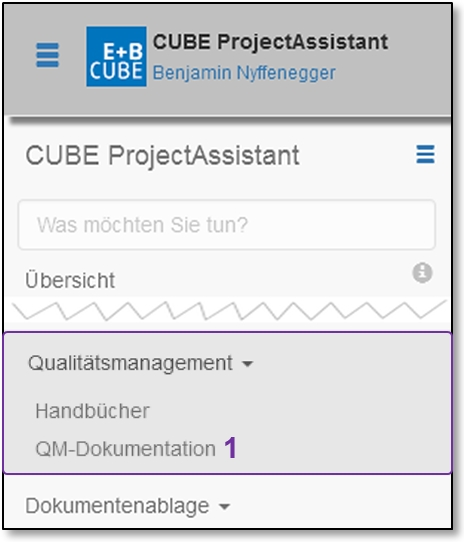
\includegraphics[width=1\linewidth]{../chapters/09_Qualitaetsmanagement/pictures/9-1_Menu_Qualitaetsmanagement.jpg}
  \end{center}
  \vspace{-20pt}
  \caption{Using quality management}
  \vspace{-10pt}
\end{wrapfigure}

Select the 'Quality Management' menu item and in this example the subcategory 'QM documentation' \col{(1)}. \\
 
\textbf{Note:} If you have several linked documents, they will all appear as subcategories under the menu time 'Quality Management'. You can choose the displayed names yourself (see chapter \ref{bkm:Ref912000789}). \\

The following view is now displayed on the right:

\vspace{6cm} 

\begin{figure}[H]
\center{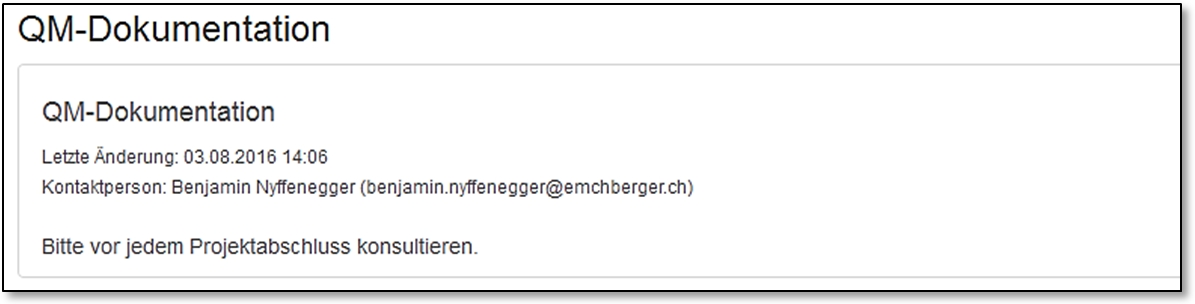
\includegraphics[width=1\linewidth]{../chapters/09_Qualitaetsmanagement/pictures/9-1_Verkn_Dokument.jpg}}
\caption{Opening a linked document}
% \label{fig:speciation}
\end{figure}

You will now see the document name and the corresponding description. You can also see who is responsible for the document and when the document was last modified, or when the document was last uploaded. By clicking on the framed field you can now open the document or save it on your computer. A dialog will be displayed, which depends on which browser you are using.

\subsubsection{Linking quality management documents}
\label{bkm:Ref912000789}

This process requires higher authorizations in CUBE PA. Contact your CUBE PA superuser or contact the CUBE PA support: {\color{red} cube.support@emchberger.ch}.

\vspace{\baselineskip}

If one (or more) document needs to be linked to 'Quality Management', proceed as follows:

\vspace{\baselineskip}

\textbf{Step 1: Create 'Data Resource Types'}

First, a new menu designation for the menu must be created (in this example the 'QM Documentation' designation was chosen). Click on the menu item 'Configuration' then on 'Data Resource Types'. You now have an overview of all existing data resource types and have the option to create a new entry using the plus symbol 
\includegraphics[height=12pt]{/Icons/Plussymbol.jpg} \col{(1)}:

\begin{figure}[H]
\center{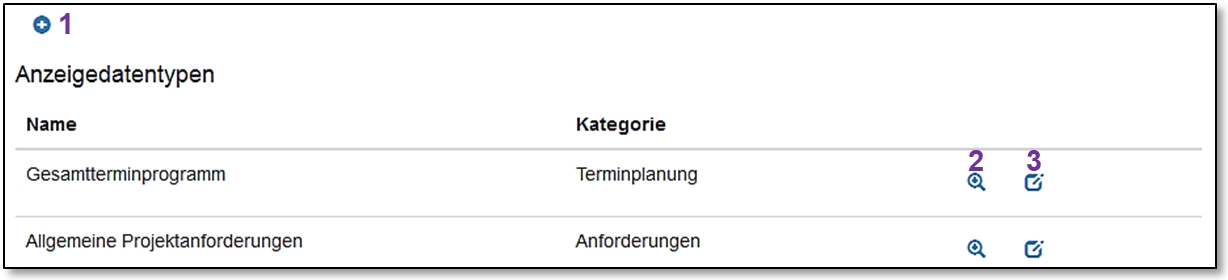
\includegraphics[width=1\linewidth]{../chapters/09_Qualitaetsmanagement/pictures/9-1-1_Anzeigedatentypen_Uebersicht.jpg}}
\caption{Data resource types overview}
% \label{fig:speciation}
\end{figure}

The magnifying glass symbol 
\includegraphics[height=12pt]{/Icons/Lupe.jpg} \col{(2)} enables you to see existing entries. The edit symbol 
\includegraphics[height=12pt]{/Icons/Bearbeiten.jpg} \col{(3)} allows you to edit an existing entry. Clicking on the plus symbol 
\includegraphics[height=12pt]{/Icons/Plussymbol.jpg} \col{(1)} enables you to access the following information and settings:

\begin{figure}[H]
\center{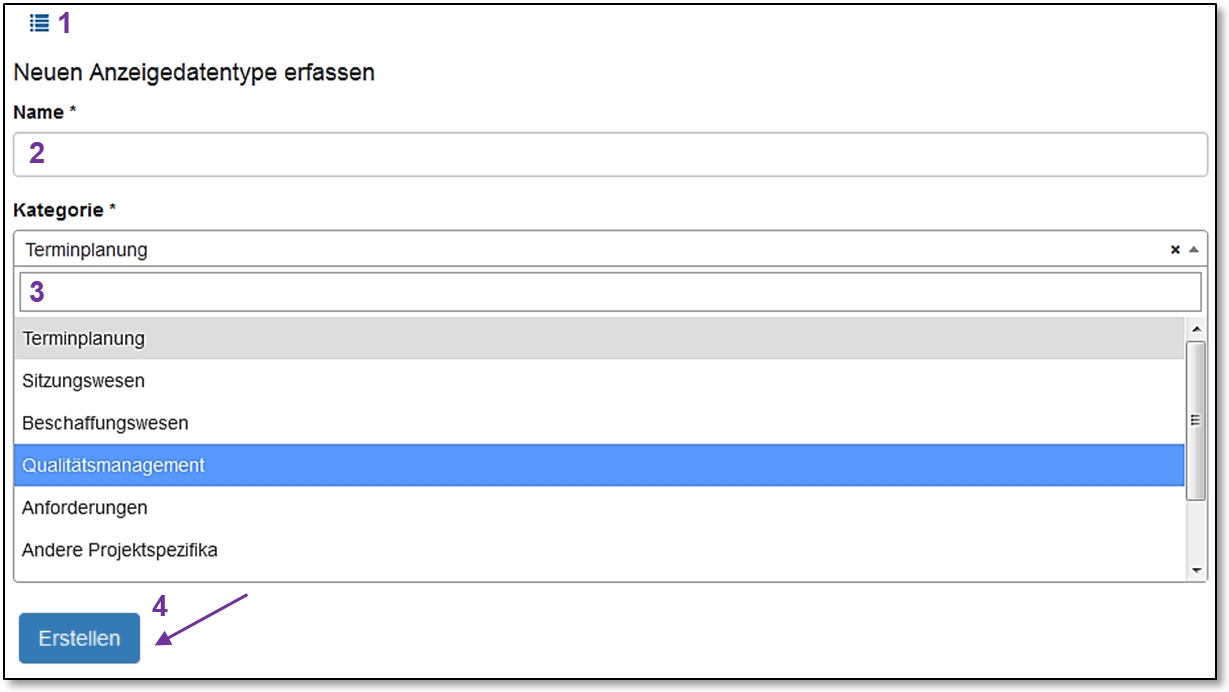
\includegraphics[width=1\linewidth]{../chapters/09_Qualitaetsmanagement/pictures/9-1-1_Anzeigedatentypen_Eingaben.jpg}}
\caption{Creating data resource types}
% \label{fig:speciation}
\end{figure}

The list symbol 
\includegraphics[height=12pt]{/Icons/Listensymbol_zurueck.jpg} \col{(1)} enables you to return to the overview. Give a meaningful name for the document link \col{(2)} (this name will then appear in the CUBE PA menu). Under 'Category' \col{(3)} in the drop-down menu select 'Quality Management' and click 'Create'. The data is saved.

\vspace{\baselineskip}

\textbf{Step 2: Create 'Data Resources'}

Now create the entry which also contains the linked document. To do so, select the 'Configuration' menu item and then 'Data Resources'. The following overview appears: 

\begin{figure}[H]
\center{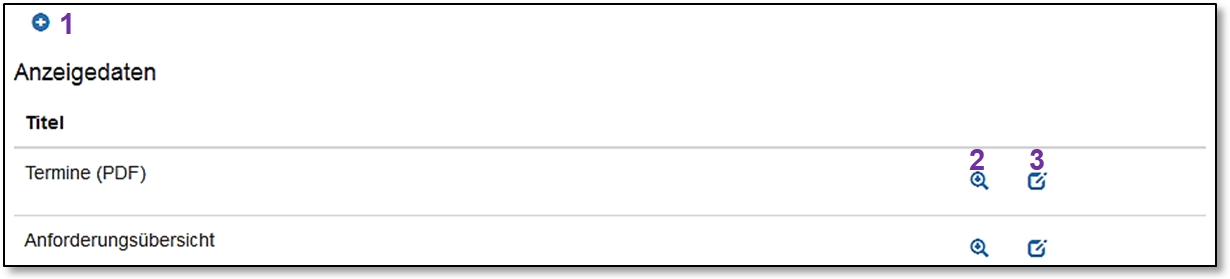
\includegraphics[width=1\linewidth]{../chapters/09_Qualitaetsmanagement/pictures/9-1-1_Anzeigedaten_Uebersicht.jpg}}
\caption{Data resources overview}
% \label{fig:speciation}
\end{figure}

You can make a new entry by clicking on the plus symbol 
\includegraphics[height=12pt]{/Icons/Plussymbol.jpg} \col{(1)}. With the magnifying glass symbol 
\includegraphics[height=12pt]{/Icons/Lupe.jpg} \col{(2)} or the edit symbol 
\includegraphics[height=12pt]{/Icons/Bearbeiten.jpg} \col{(3)} you can view or edit an existing entry. By clicking on the plus symbol 
\includegraphics[height=12pt]{/Icons/Plussymbol.jpg} \col{(1)} a new document link is created. 

\begin{figure}[H]
\center{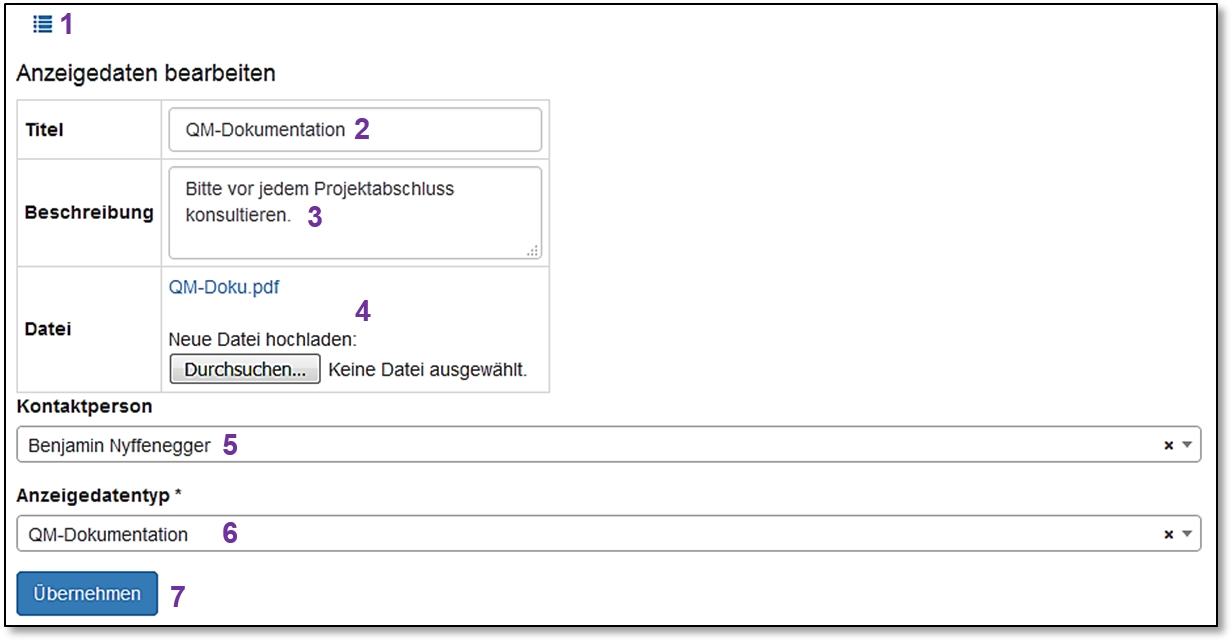
\includegraphics[width=1\linewidth]{../chapters/09_Qualitaetsmanagement/pictures/9-1-1_Anzeigedaten_Eingaben.jpg}}
\caption{Creating data resources}
% \label{fig:speciation}
\end{figure}

The list symbol 
\includegraphics[height=12pt]{/Icons/Listensymbol_zurueck.jpg} \col{(1)} enables you to return to the overview. Enter the desired title \col{(2)} (possibly the same one used for the 'Data Resource Type'). You can now add a description \col{(2)}, which will be displayed under 'Quality Management' and the corresponding / created menu item. Under 'File' \col{(4)}, the desired document is uploaded and linked. Click on 'Browse' and select desired file in the Explorer window.\\

You can optionally select contact persons \col{(5)}. They are also displayed with their stored e-mail addresses. Now the 'Data Resources' are linked with the desired 'Data Resource Types' \col{(6)}. Click on 'Apply', and the data will be saved. The preparation work is now done. The linked document can now be opened under the 'Quality Management' menu item and the corresponding sub-item. For a better overview of which data is displayed, here is the document entry with comments:

\begin{figure}[H]
\center{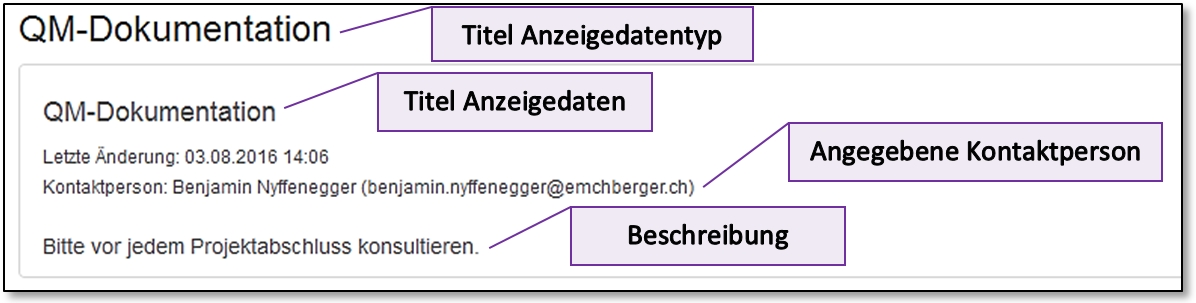
\includegraphics[width=1\linewidth]{../chapters/09_Qualitaetsmanagement/pictures/9-1-1_AngezeigteDaten.jpg}}
\caption{Data Resource Types under Quality Management}
% \label{fig:speciation}
\end{figure}

If the linked document changes, you can edit the existing entry and simply upload the new file. The 'Last update' will be accordingly updated and the new file will be available.

\subsection{Project handbook}

\begin{wrapfigure}[6]{l}{6.5cm}   % [x] Wie manche Zeile soll sich um die Grafik "brechen"
  \vspace{-35pt}      % Grundwert war 20; mit 30 schön oben beim Text ausgerichtet
  \begin{center}
    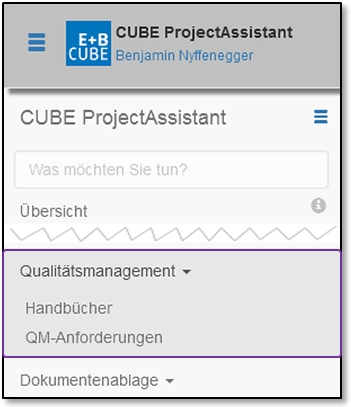
\includegraphics[width=1\linewidth]{../chapters/09_Qualitaetsmanagement/pictures/9-2_Menu_Qualitaetsmanagement_Handbuch.jpg}
  \end{center}
  \vspace{-20pt}
  \caption{The handbook function in CUBE PA}
  \vspace{-10pt}
\end{wrapfigure}

In quality management, you can design handbooks, like for example a project handbook. To do so click the 'Handbooks' sub-item in the menu.

\vspace{2.5cm}  

If you have already added handbooks, these will be listed in the following overview:\\

\vspace{3cm}  

\begin{figure}[H]
\center{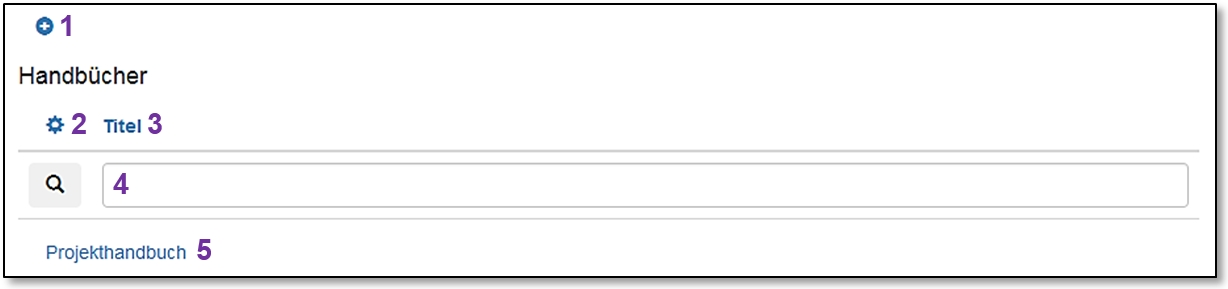
\includegraphics[width=1\linewidth]{../chapters/09_Qualitaetsmanagement/pictures/9-2_Handbuch_Uebersicht.jpg}}
\caption{Overview of the handbooks}
% \label{fig:speciation}
\end{figure}

You can create a new Handbook by clicking on the plus symbol 
\includegraphics[height=12pt]{/Icons/Plussymbol.jpg} \col{(1)} (see chapter \ref{bkm:Ref930000788}). The configuration symbol 
\includegraphics[height=12pt]{/Icons/SpaltenEinst.jpg} \col{(2)} enables you to show or hide columns (This can't be changed in the handbook overview since there's only one column). Clicking on the blue title \col{(3)} sorts the listed handbooks from A to Z. Clicking again sorts them from Z to A. If you are looking for a specific handbook, you can enter a certain term in the search field \col{(4)} and then click on the magnifying glass symbol 
\includegraphics[height=12pt]{/Icons/Lupe_s.jpg} or hit 'Enter'. The filtered document / handbook list appears. (Warning: The filter currently only searches through the handbook titles and not their content). Click on a handbook \col{(5)} to open it:

\begin{figure}[H]
\center{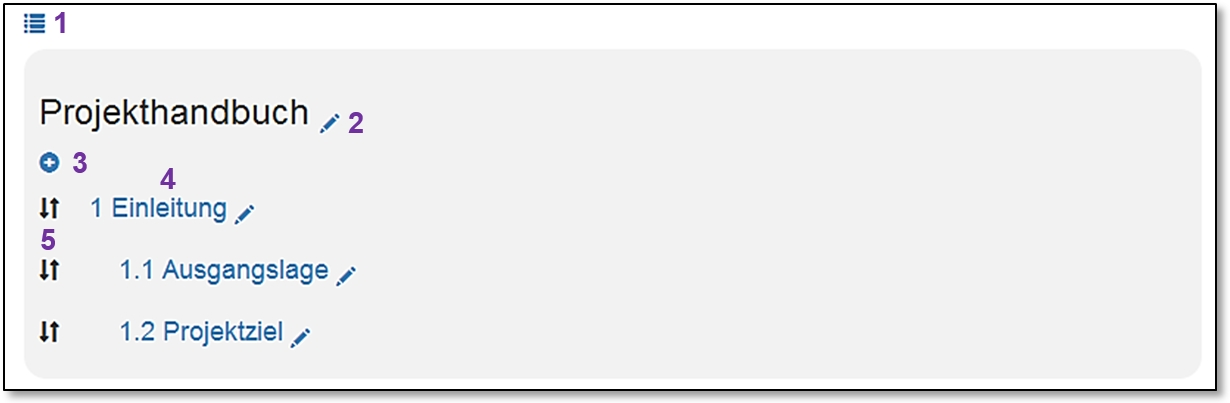
\includegraphics[width=.75\linewidth]{../chapters/09_Qualitaetsmanagement/pictures/9-2_Projekthandbuch.jpg}}
\caption{A handbook outline}
% \label{fig:speciation}
\end{figure}

Click on the list symbol 
\includegraphics[height=12pt]{/Icons/Listensymbol_zurueck.jpg} \col{(1)} to return to the overview of handbooks. You can edit the entry by clicking on the pen symbol 
\includegraphics[height=12pt]{/Icons/Stift.jpg} \col{(2)} and you can add a new chapter by clicking on the plus symbol 
\includegraphics[height=12pt]{/Icons/Plussymbol.jpg} \col{(3)}. If you click on a blue title \col{(4)}, the chapter is opened. If you need to change the chapter order, drag the vertical opposing arrows symbol 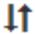
\includegraphics[height=12pt]{/Icons/VertPfeile.jpg} \col{(5)} next to a chapter and drop it at the desired position. \\
You have the possibility to save the entire handbook as a PDF document. To do so, click on the download symbol 
\includegraphics[height=12pt]{/Icons/Download.jpg} \col{(6)}. A zip-file containing the PDF handbook and any linked documents.

\subsubsection{Editing an existing handbook}

The title of a handbook can be changed in the outline (by clicking on the pen symbol 
\includegraphics[height=12pt]{/Icons/Stift.jpg} \col{(2)}). After making the changes click the check-mark next to the title to save the changes:

\begin{figure}[H]
\center{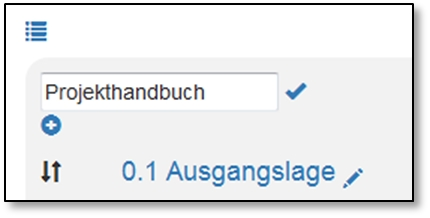
\includegraphics[width=0.35\linewidth]{../chapters/09_Qualitaetsmanagement/pictures/9-2-1_HandbuchTitel_aendern.jpg}}
\caption{Changing the title of a handbook}
% \label{fig:speciation}
\end{figure}

To change an entry, click on the pen symbol 
\includegraphics[height=12pt]{/Icons/Stift.jpg} next to the desired chapter. The following input form appears:

\begin{figure}[H]
\center{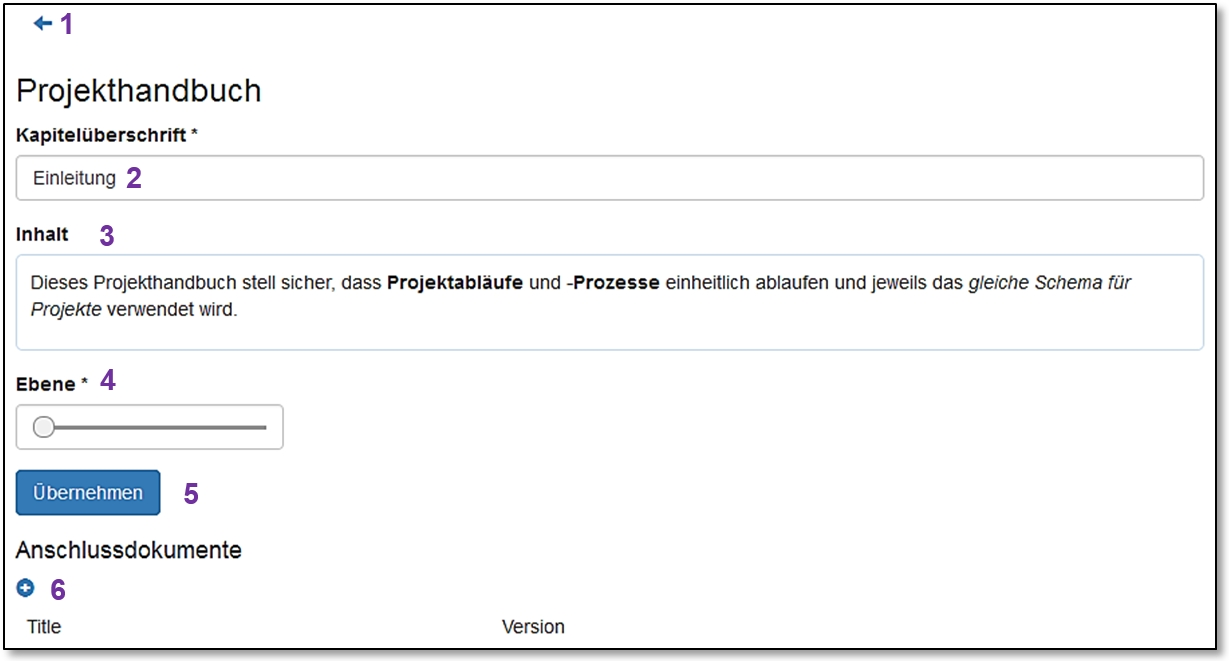
\includegraphics[width=1\linewidth]{../chapters/09_Qualitaetsmanagement/pictures/9-2-1_Handbuch_aendern.jpg}}
\caption{Editing a chapter}
% \label{fig:speciation}
\end{figure}

Click the arrow symbol 
\includegraphics[height=12pt]{/Icons/Pfeil-links.jpg} \col{(1)} to return to the handbook (outline). In the different input fields you can see the existing entries which can now be modified. You can change a chapter title \col{(2)} (the chapter title is a mandatory field and must be / stay filled). You can edit the content \col{(3)} of a chapter. The level bar \col{(4)} enables you to change the chapter hierarchy. Move the slider to the left to put a chapter in the first level (1), to the middle to put it in the first lower level (1.1), and to the right to put it in the second lower level (1.1.1). \\

Documents can be assigned to specific chapters. Click on the plus symbol 
\includegraphics[height=12pt]{/Icons/Plussymbol.jpg} \col{(6)} to get an overview of the related documents:

\begin{figure}[H]
\center{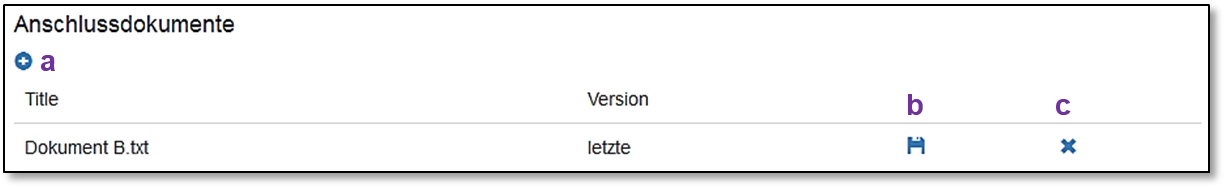
\includegraphics[width=1\linewidth]{../chapters/09_Qualitaetsmanagement/pictures/9-2-1_Anschlussdokumente_aendern.jpg}}
\caption{Related documents}
% \label{fig:speciation}
\end{figure}

You can add a document by clicking the plus symbol 
\includegraphics[height=12pt]{/Icons/Plussymbol.jpg} \col{(a)}. You can save an existing document on your computer by clicking the save symbol 
\includegraphics[height=12pt]{/Icons/Diskette.jpg} \col{(b)} or remove it by clicking on the cross 
\includegraphics[height=12pt]{/Icons/Kreuzchen.jpg} \col{(c)}.

Click 'Apply' \col{(5)} to save changes. 

\subsubsection{Creating a new handbook}
\label{bkm:Ref930000788}

To create a new handbook, proceed as follows:

Select the 'Quality Management' menu item and then 'Handbooks'. In the overview of handbooks click on the plus symbol 
\includegraphics[height=12pt]{/Icons/Plussymbol.jpg} \col{(1)}.

\begin{figure}[H]
\center{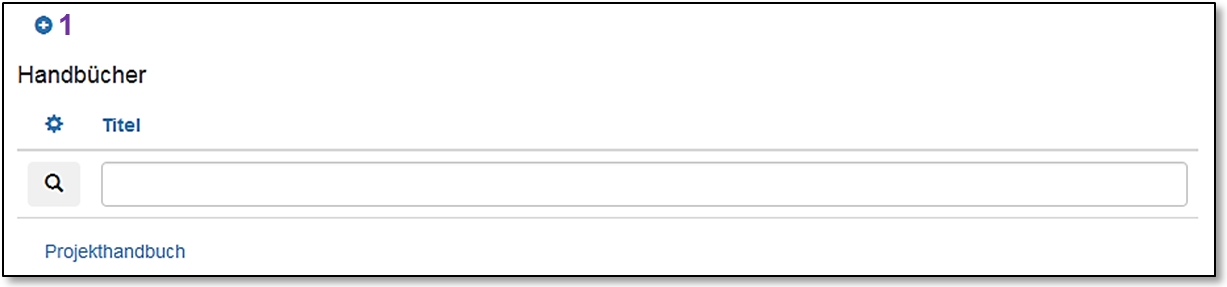
\includegraphics[width=1\linewidth]{../chapters/09_Qualitaetsmanagement/pictures/9-3-2_NeuesHandbuch_erstellen.jpg}}
\caption{Creating a new handbook}
% \label{fig:speciation}
\end{figure}

Enter a title for the new handbook: 

\begin{figure}[H]
\center{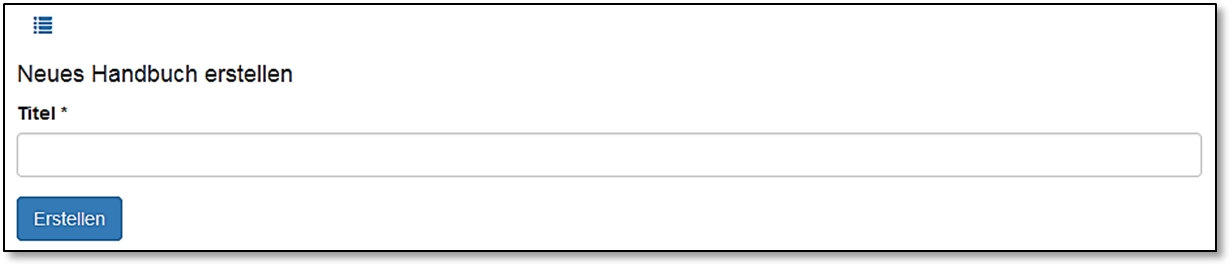
\includegraphics[width=1\linewidth]{../chapters/09_Qualitaetsmanagement/pictures/9-3-2_Handbuch_erstellen_Titel.jpg}}
\caption{Creating a new handbook - Entering a title}
% \label{fig:speciation}
\end{figure}

Then click on the 'Create' button. The handbook now exists.

\begin{figure}[H]
\center{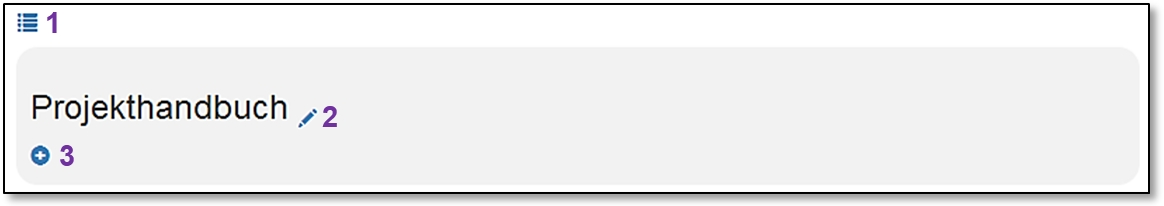
\includegraphics[width=.8\linewidth]{../chapters/09_Qualitaetsmanagement/pictures/9-3-2_Handbuch_angelegt.jpg}}
\caption{New handbook - Adding chapters}
% \label{fig:speciation}
\end{figure}

The list symbol 
\includegraphics[height=12pt]{/Icons/Listensymbol_zurueck.jpg} \col{(1)} enables you to return to the overview of handbooks. You can change the tile of the handbook by clicking on the pen symbol 
\includegraphics[height=12pt]{/Icons/Stift.jpg} \col{(2)}. Click the plus symbol 
\includegraphics[height=12pt]{/Icons/Plussymbol.jpg} \col{(3)} to add chapters:

\begin{figure}[H]
\center{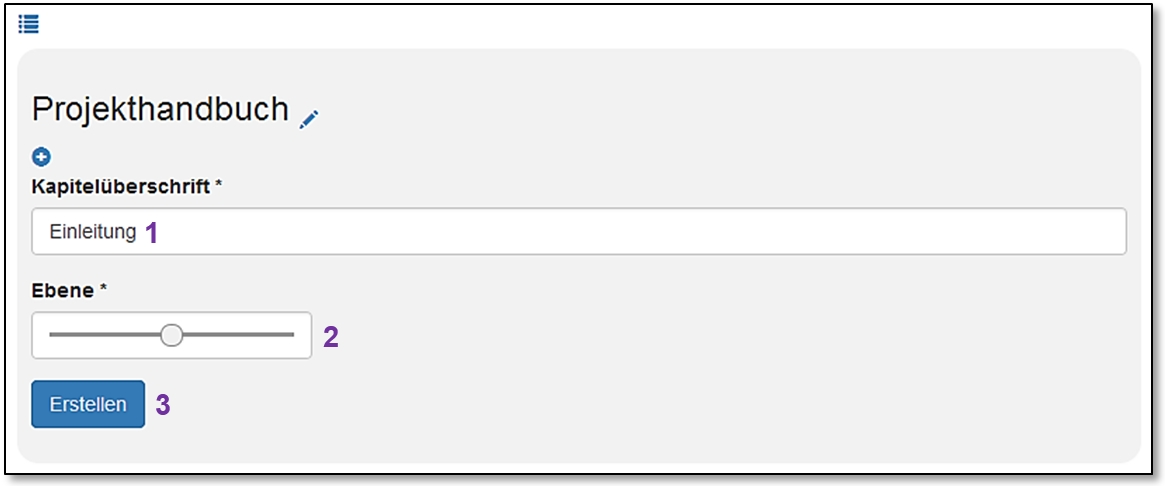
\includegraphics[width=.8\linewidth]{../chapters/09_Qualitaetsmanagement/pictures/9-3-2_Kapitel_anlegen.jpg}}
\caption{New handbook - Naming chapters}
% \label{fig:speciation}
\end{figure}

Enter the desired chapter title \col{(1)}. You have the possibility to set the chapter level (Left: 1, Middle: 1.1, Right: 1.1.1). The chapter level can be changed at a later stage. Once you've entered the required information and chosen the required settings, click on 'Create'. The chapter is added and the input form changes:

\begin{figure}[H]
\center{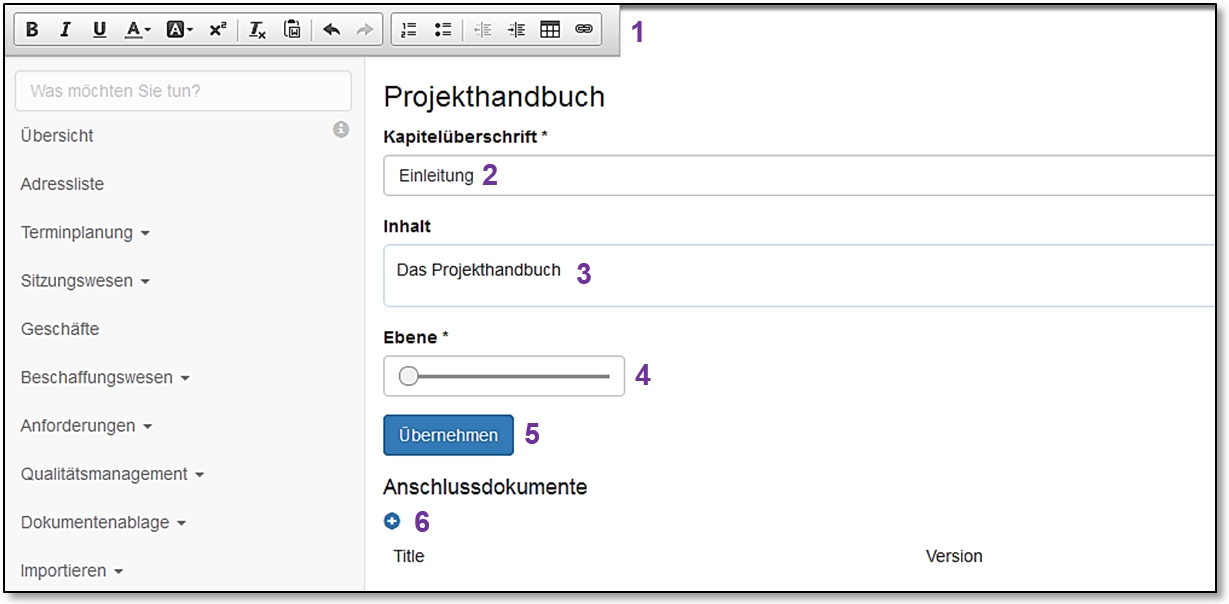
\includegraphics[width=1\linewidth]{../chapters/09_Qualitaetsmanagement/pictures/9-2-3_Kapitel_bearbeiten.jpg}}
\caption{New handbook - Editing chapters}
% \label{fig:speciation}
\end{figure}

You can still change the chapter title \col{(2)}. When you click in the 'Content' field \col{(3)} a menu \col{(1)} appears at the top left. This menu enables you to format text, insert tables, or undo changes. More information is given below. You can also change the chapter level with the level bar \col{(4)}. All changes need to be saved by clicking on the 'Apply' button \col{(5)}. An additional function now appears: you can add documents or links to chapters \col{(6)}. To do so, click on the plus symbol 
\includegraphics[height=12pt]{/Icons/Plussymbol.jpg} \col{(6)}: 

\begin{figure}[H]
\center{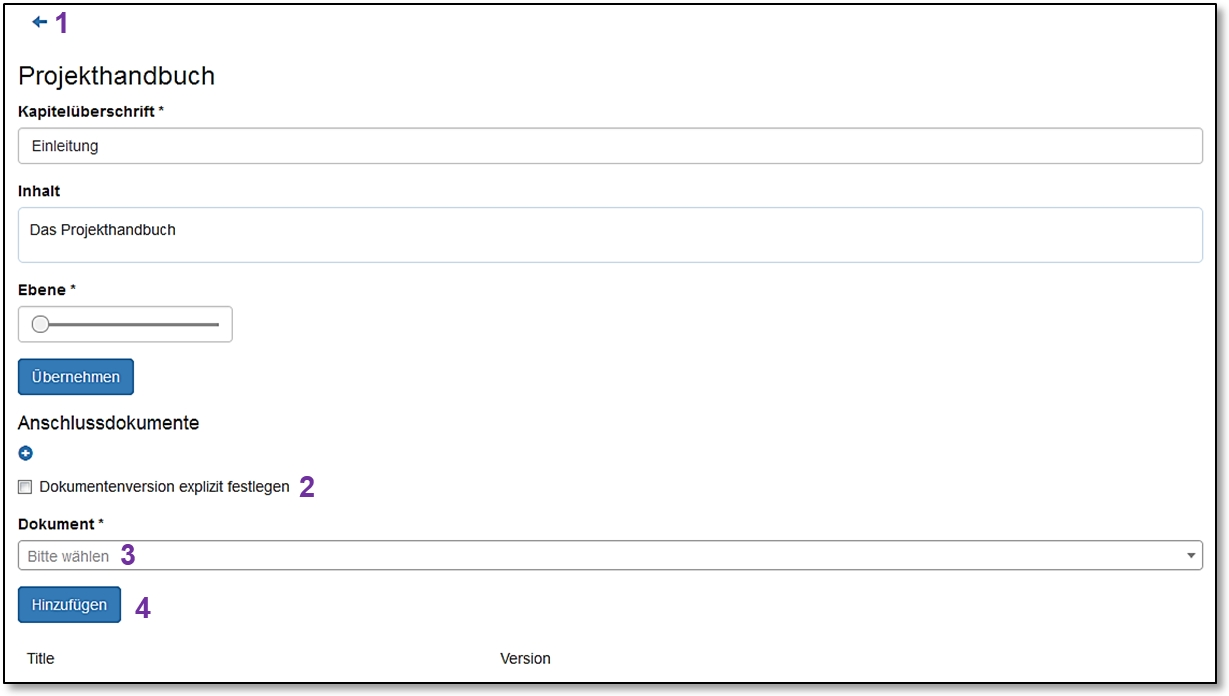
\includegraphics[width=1\linewidth]{../chapters/09_Qualitaetsmanagement/pictures/9-3-2_Kapitel_Dokumente_hinzufuegen.jpg}}
\caption{New handbook - Adding documents}
% \label{fig:speciation}
\end{figure}

When creating or editing a handbook, you return to the handbook outline by clicking on the arrow symbol 
\includegraphics[height=12pt]{/Icons/Pfeil-links.jpg} \col{(1)}. However, your changes will be lost if you didn't click the 'Apply' button first. If you're in the 'Content' text field, the arrow symbol will be covered. Click for example in the chapter title field to make the arrow symbol visible again. \\

\textbf{Linking documents:} At the bottom of the window you have the possibility to select a document and to link it to the chapter. All documents uploaded in the CUBE PA document management function are available for selection. If you want to link to a new document while working on a handbook, save your changes by clicking on the 'Apply' button and then go to 'Document Management' in the main menu to first upload the desired document to CUBE PA. More information about uploading documents can be found in chapter \ref{bkm:Ref442863508}. \\

The 'Explicitly set document version' function \col{(2)} enables you to link to a specific version of a document. If you don't use this function, the most recent version of the document found in document management will appear / be linked to in the handbook chapter. There are situations which require that a specific version of a document remains linked. To do so, click on the small check-box to activate the function. More information about document management and the versions of documents can be found in chapter \ref{bkm:Ref443047930}. \\

Repeat the above steps to link to more documents. \\

\textbf{Text formatting and other functions:}

\begin{figure}[H]
\center{\includegraphics[width=.8\linewidth]{../chapters/09_Qualitaetsmanagement/pictures/9-2-3_Text_formatieren.jpg}}
\caption{New handbook - Text formatting}
% \label{fig:speciation}
\end{figure}

As with a word processing software, the chapter content can be formatted, tables can be inserted, and links to websites can be added. The following is an overview of the different available functions: \\

\begin{tabular}{c | p{14cm} l} %{cl}
\hline
\includegraphics[height=12pt]{../chapters/09_Qualitaetsmanagement/pictures/Format/Fett.jpg} & The text is displayed in bold \\
\hline
\includegraphics[height=12pt]{../chapters/09_Qualitaetsmanagement/pictures/Format/Kursiv.jpg} & The text is displayed in italics \\
\hline
\includegraphics[height=12pt]{../chapters/09_Qualitaetsmanagement/pictures/Format/Unterstrichen.jpg} & The text is underlined \\
\hline
\includegraphics[height=12pt]{../chapters/09_Qualitaetsmanagement/pictures/Format/Textfarbe.jpg} & The text color can be changed \\
\hline
\includegraphics[height=12pt]{../chapters/09_Qualitaetsmanagement/pictures/Format/Hintergrundfarbe.jpg} & The background color of the text can be changed \\
\hline
\includegraphics[height=12pt]{../chapters/09_Qualitaetsmanagement/pictures/Format/Form_z.jpg} & The text formatting is removed \\
\hline
\includegraphics[height=12pt]{../chapters/09_Qualitaetsmanagement/pictures/Format/ausWord.jpg} & Content located in the clipboard, for example from Word, can be added. (A message appears if the browser does not support this function. However, you still have the option to paste selected text in the box that appears and to transfer it into CUBE PA.) \\
\hline
\includegraphics[height=12pt]{../chapters/09_Qualitaetsmanagement/pictures/Format/Undo.jpg} & The 'undo' function undoes the last change and the 'redo' function restores an undone change \\
\hline
\includegraphics[height=12pt]{../chapters/09_Qualitaetsmanagement/pictures/Format/Aufzaehlung.jpg} & Text is converted into a numbered list or a list with bullets \\
\hline
\includegraphics[height=12pt]{../chapters/09_Qualitaetsmanagement/pictures/Format/Einruecken.jpg} & The indent of a text is reduced (text is moved to the left) or increased (text is moved to the right) \\
\hline
\includegraphics[height=12pt]{../chapters/09_Qualitaetsmanagement/pictures/Format/Tabellen.jpg} & Inserts tables. Tables can be captioned and formatted (borders, size, direction, etc.) \\
\hline
\includegraphics[height=12pt]{../chapters/09_Qualitaetsmanagement/pictures/Format/Link.jpg} & Links to websites or text markers within the handbook text can be made. E-mail addresses can also be included in the handbook.\\
\hline
\end{tabular}

% bishierher




